\documentclass{beamer}
\usepackage[utf8]{inputenc}
\usepackage{amsmath}
\usepackage{amsfonts}
\usepackage{amssymb}
\usepackage{graphics}
\usepackage{wrapfig}
\usepackage{hyperref}
\usepackage{float}
\usepackage{tikz}
\usepackage{xurl}

\tikzstyle{arrow} = [thick,->,>=stealth]


\usetheme{Madrid}

\title{Digital Recognition}
\subtitle{Min Project prepared for Dr. Youssef HARKOUS}
\author{Ali El Hadi ISMAIL FAWAZ}
\institute[LUFE]
{Lebanese University \and Faculty of Engineering branch III - Hadath \and Department of Electrical and Telecommunication Engineering}
\date[\today]
{4th Year - Semester 7 - Fall 2020/2021 - \today}
\logo{
\includegraphics[scale=0.1]{ulfg_logo.png}}

\AtBeginSection[]
{
	\begin{frame}
		\frametitle{Table of Contents}
		\tableofcontents[currentsection]
	\end{frame}
}

\begin{document}

\frame{\titlepage}

\begin{frame}
\frametitle{Table of Contents}
\tableofcontents
\end{frame}

\section*{Acknowledgments}
\begin{frame}
\frametitle{Acknowledgments}
First and foremost, we would like to thank the dean, the faculty director, the head of the electrical and
telecommunication department and of course Dr. Y. Harkous for whom we are presenting our work.
\end{frame}

\section{Introduction}

\begin{frame}
\frametitle{Introduction}
\begin{block}{What is Artificial Intelligence (AI).}
\large “ The science and engineering of making intelligent machines, especially intelligent computer programs ”. -John McCarthy-
\end{block}

\begin{figure}
\centering
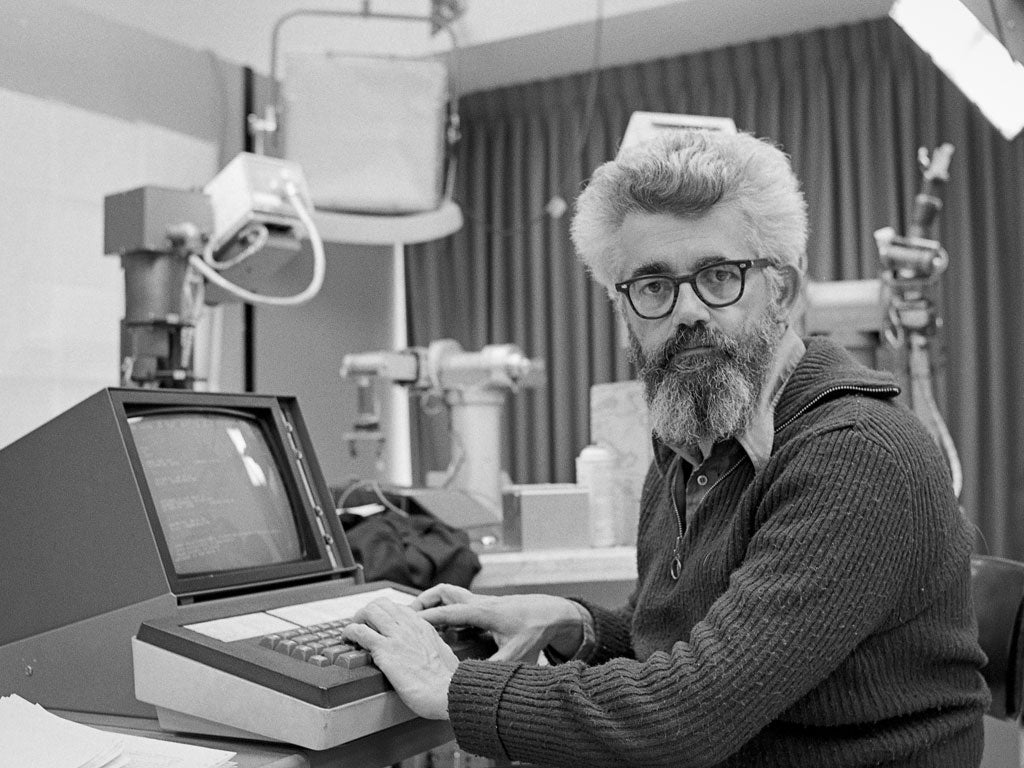
\includegraphics[scale=0.15]{John-McCarthy.jpg}
\caption{\url{https://www.independent.co.uk/news/obituaries/john-mccarthy-computer-scientist-known-father-ai-6255307.html}}
\end{figure}

\end{frame}

\begin{frame}
\frametitle{Introduction}
\begin{block}{AI VS HI}
Which is better and by how much, Artificial or Human Intelligence.
\end{block}
\begin{figure}
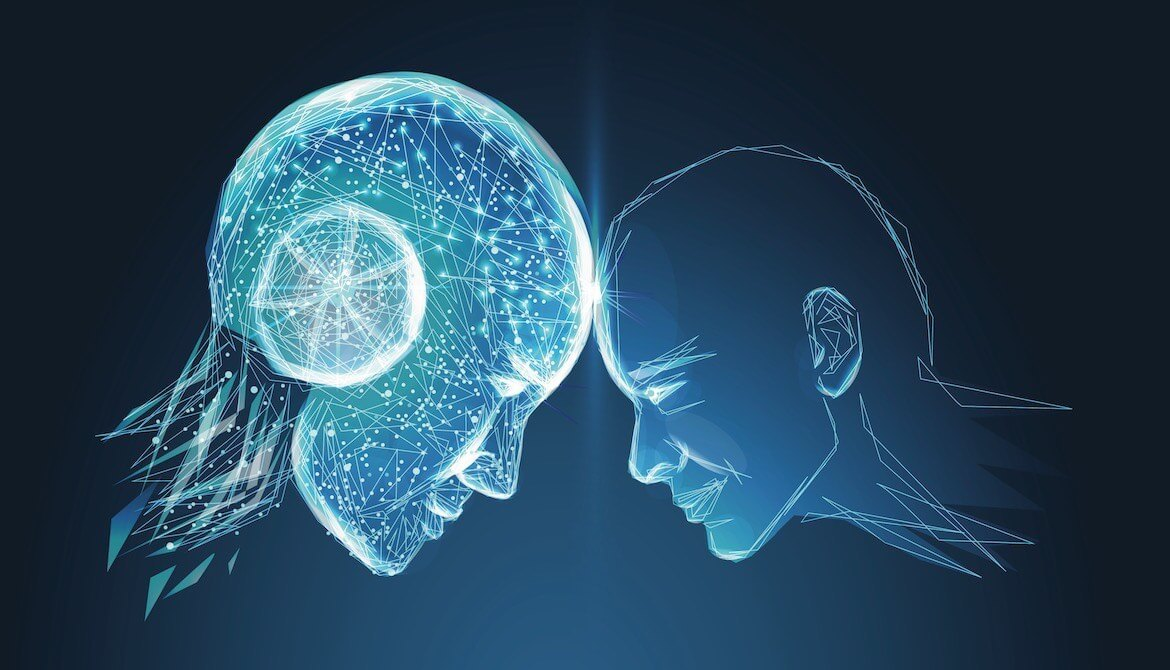
\includegraphics[scale=0.2]{AI_VS_HI.jpg}
\caption{\url{https://www.cumanagement.com/articles/2018/09/humans-versus-ai}}
\end{figure}
\end{frame}

\section{Materials Used}

\begin{frame}
\frametitle{Materials Used}
\begin{block}{Programming language and modules}
\begin{itemize}
\item Python (version 3.8.5)
\begin{itemize}
\item Tkinter module for the Graphical User interface
\item Keras module for the data and deep learning.
\item Tslearn for nearest neighbor algorithm
\item Sklearn for the used metrics
\end{itemize}
\end{itemize}
\end{block}

\end{frame}

\begin{frame}
\frametitle{Materials Used}
\begin{figure}
\centering 
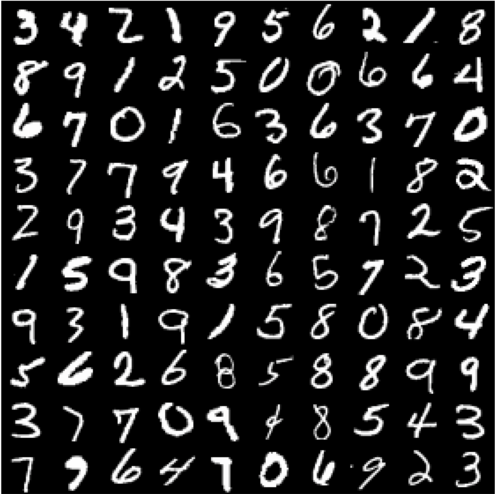
\includegraphics[scale=0.35]{mnist.png}
\caption{Mnist Data Set \textcolor{blue}{\href{https://medium.com/@ankitbatra2202/mnist-handwritten-digit-recognition-with-pytorch-cce6a33cd1c1}{Link}}}
\end{figure}
\end{frame}

\section{Data Normalization}

\begin{frame}
\frametitle{Data Normalization}
Data normalization is considered a very essential part of machine learning and deep learning, why is that?
\begin{block}{Types of normalization}
\begin{itemize}
\item \small Z-Normalization : $ x^{\prime} = \dfrac{x - \mu}{\sigma} $ , $ \mu = \dfrac{1}{n}\sum_{i=1}^{i=n}x_i $ $ \sigma = \sqrt{\dfrac{1}{n-1}\sum_{i=1}^{i=n}(x_i - \mu)^2} $
\item Min-Max-Normalization : $ x^{\prime} = \dfrac{x - \min{(x)}}{\max{(x)} - \min{(x)}} $
\item Unit-Vector-Normalization : $ \vec{x^{\prime}} = \dfrac{\vec{x}}{||\vec{x}||} $ , $ ||\vec{x^{\prime}}|| = 1 $
\end{itemize}
\end{block}
\end{frame}

\section{Train Test Split}

\begin{frame}
\frametitle{Train Test Split}
What is train test split and why do we need it?
\begin{figure}
\centering
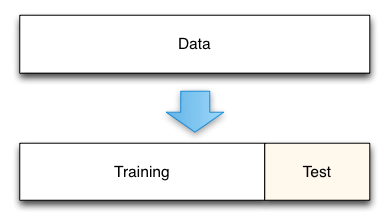
\includegraphics[scale=0.4]{Train-Test-Data-Split.png}
\caption{Train Test Split \textcolor{blue}{\href{https://www.researchgate.net/figure/Train-Test-Data-Split_fig6_325870973}{Link}}}
\end{figure}
\end{frame}

\section{Nearest Neighbor}

\begin{frame}
\frametitle{Nearest Neighbor}
\begin{alertblock}{Note :}
The real name of this algorithm is K-Nearest-Neighbor (K-NN), K being the number of the nearest neighbors of an instance, in our project $ K = 1 $ .
\end{alertblock}
K-NN is a basic algorithm to solve classification problems.
\begin{block}{K-NN has two steps :}
\begin{itemize}
\item Given an instance and a data set, find the K nearest neighbors of this instance from the data set
\item Classify the instance as the most dense class in its neighbors
\end{itemize}
\end{block}
\end{frame}

\begin{frame}
\frametitle{Nearest Neighbor}
\begin{example}

We are classifying an instance $ x $ with $ K = 3 $ based on a data set $ \{y_0,y_1,y_2,...,y_n\} $ and we found that $ y_0, y_1 $ and $ y_2 $ are the 3 nearest neighbors of $ x $. If $ y_0 $ and $ y_2 $ are classified as $ c_0 $ and $ y_1 $ as $ c_1 $, $ x  $ would be classified then as $ c_0 $ as it is the most dense class in the nearest neighbors of $ x $.

\end{example}
\begin{alertblock}{Note :}
If $ K = 1 $, then $ x $ would be classified as its one and only nearest neighbor.
\end{alertblock}
\begin{block}{How to find the nearest neighbor of an instance ?}
To find the nearest neighbor we just have to calculate the distance of the vector $ x $ to all the instances in the data set and $ x $'s nearest neighbor would be the instance with the smallest distance from it, here we will talk about two distances.
\end{block}
\end{frame}

\begin{frame}
\frametitle{Nearest Neighbor - Euclidean Distance (ED)}
\begin{columns}

\column{0.6\textwidth}
\begin{itemize}
\item In a two dimensional space the euclidean distance between two points is :\\
$ ED(x,y) = \sqrt{(x_1 - y_1)^2 + (x_2 - y_2)^2} $
\item In a N-dimensional space : \\
$ ED(x,y) = \sqrt{\sum_{i=1}^{i=n}(x_i - y_i)^2} $
\end{itemize}
\column{0.4\textwidth}
\centering
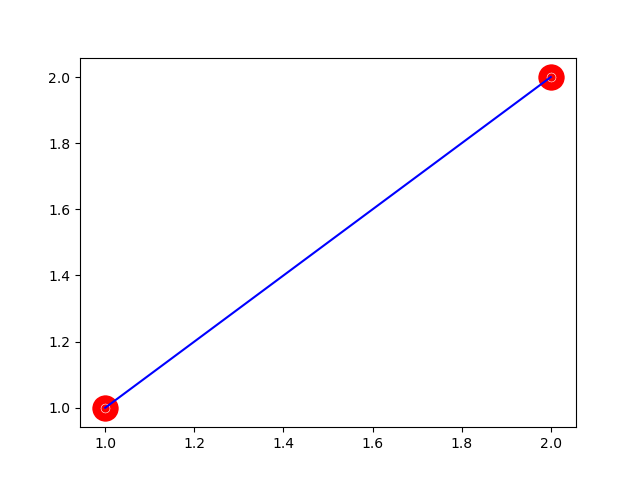
\includegraphics[scale=0.3]{ED.png}
\end{columns}
\begin{alertblock}{Note :}
Using the euclidean distance we must assert that $ x $ and $ y $ have the same length.
\end{alertblock}

\end{frame}

\begin{frame}
\frametitle{Nearest Neighbor - Dynamic Time Warping (DTW)}
\begin{block}{What is DTW ?}
DTW is an algorithm to find the similarity between two time series.\\
So lets explain what is a time series.
\end{block}
\begin{figure}
\centering
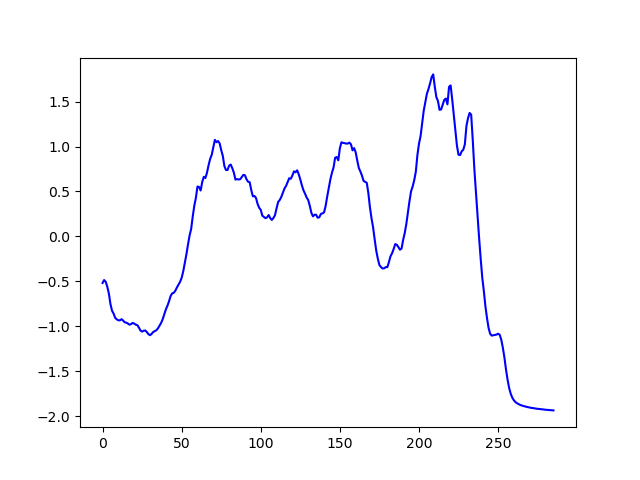
\includegraphics[scale=0.4]{Coffee.png}
\caption{Time Series of the Coffee Data Set from UCR Archive \textcolor{blue}{\href{https://www.cs.ucr.edu/~eamonn/time_series_data_2018/}{Link}}}
\end{figure}

\end{frame}

\begin{frame}
\frametitle{Nearest Neighbor - Dynamic Time Warping (DTW)}
To explain more about DTW and how it works, lets consider an example of two time series :
\begin{example}
$ x = [5,3,4,0,1,3,5,0,2,1] $ and $ y = [11,12,11,8,9,11,12,9,11,10] $
\begin{columns}
\column{0.5\textwidth}
\centering
\begin{figure}
\centering
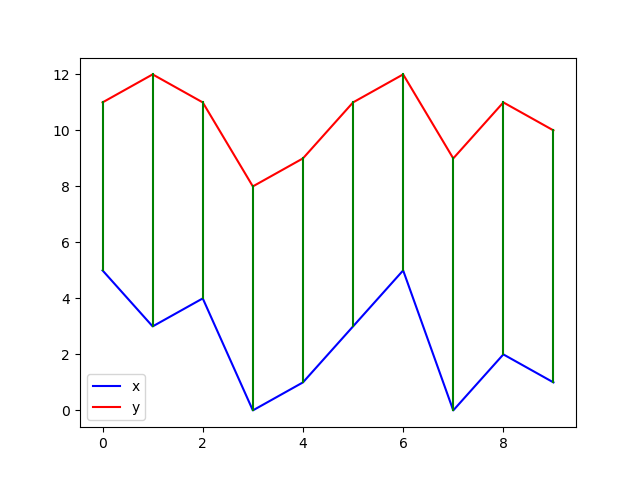
\includegraphics[scale=0.3]{ED_TS.png}
\caption{(a) - Euclidean Distance}
\end{figure}
\column{0.5\textwidth}
\centering
\begin{figure}
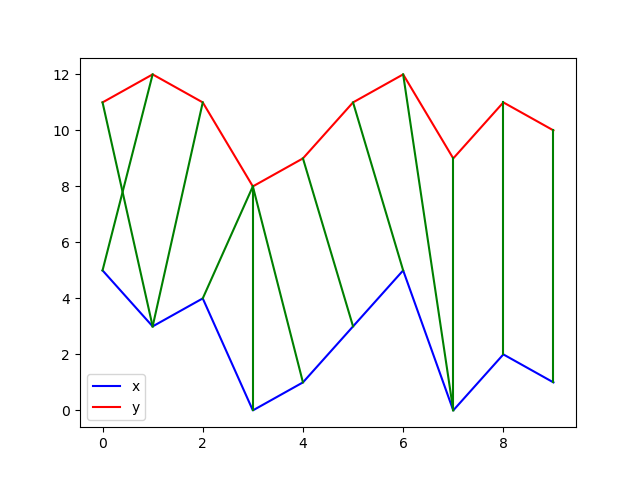
\includegraphics[scale=0.3]{DTW_TS.png}
\caption{(b) - Dynamic Time Warping}
\end{figure}
\end{columns}
\end{example}
\end{frame}

\begin{frame}
\frametitle{Nearest Neighbor - Dynamic Time Warping (DTW)}
\begin{block}{So how to calculate this optimal distance between $ x $ of length $ n $ and $ y $ of length $ m $ ?}
\begin{itemize}
\item Step 1 : Define a $ (n+1)*(m+1) $ matrix $ A $.
\item Step 2 : We set $ A[0][0]=0,A[0][1:m]=\infty $ and $ A[1:n][0]=\infty $.
\item Step 3 : For each cell $ (i,j) $ we find $ cost = (x[i-1]-y[j-1])^2 $ and $ A[i][j]=cost+\min(A[i-1][j],A[i][j-1],A[i-1][j-1]) $.
\item Step 4 : $ DTW(x,y)=\sqrt{A[n][m]} $.
\end{itemize}
\end{block}
\end{frame}

\begin{frame}
\frametitle{Nearest Neighbor - Dynamic Time Warping (DTW)}
\begin{figure}
\centering
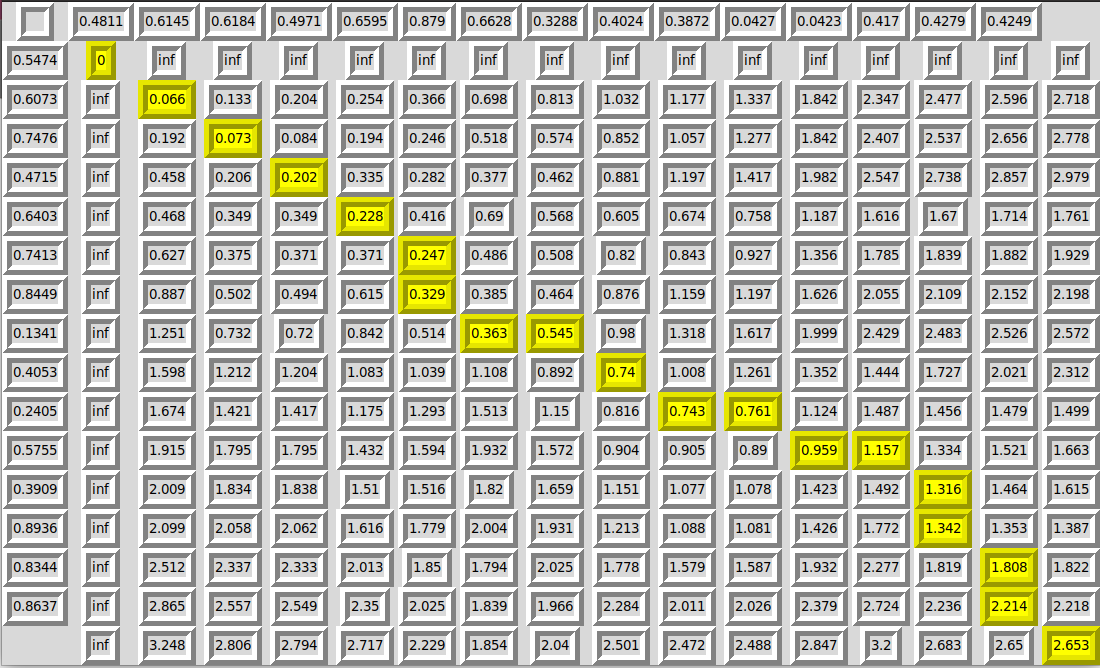
\includegraphics[scale=0.27]{DTW_GUI.png}
\caption{DTW between 2 time series of the data set "SmoothSubspace" of the UCR Archive.}
\end{figure}
\end{frame}

\section{Neural Networks}


\begin{frame}
\frametitle{Neural Networks}
Or what we call "deep learning" methods.
Why is it called Neural Networks and what is the difference between a Human Brain and an Artificial one ?
\begin{columns}
\column{0.5\textwidth}
\centering
\begin{figure}
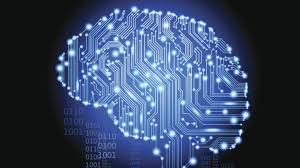
\includegraphics[scale=0.55]{artificial_brain.jpeg}
\caption{ - (a) Artificial Brain \textcolor{blue}{\href{https://www.thedailybeast.com/the-science-communitys-fight-over-an-artificial-brain}{Link}}}
\end{figure}
\column{0.5\textwidth}
\centering
\begin{figure}
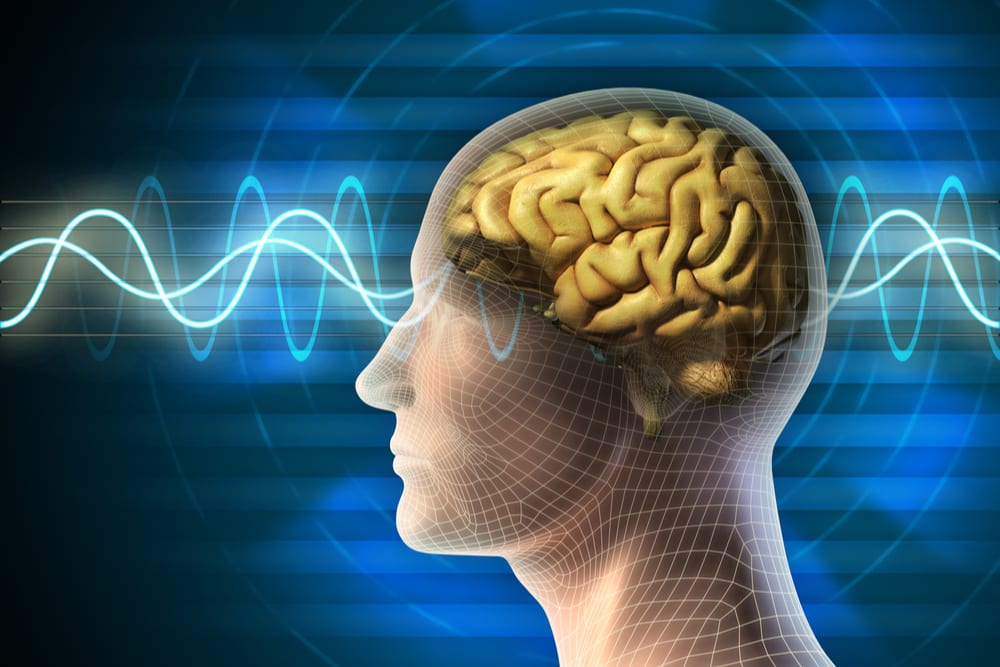
\includegraphics[scale=0.14]{humain_brain.jpg}
\caption{ - (b) Human Brain \textcolor{blue}{\href{https://www.pymnts.com/innovation/2019/elon-musk-human-brain-connected-device/}{Link}}}
\end{figure}
\end{columns}
\end{frame}

\begin{frame}
\frametitle{Neural Networks - Artificial Neurons}
\begin{block}{What is an artificial neuron ?}
It is simply a linear input output system
\end{block}
\begin{center}
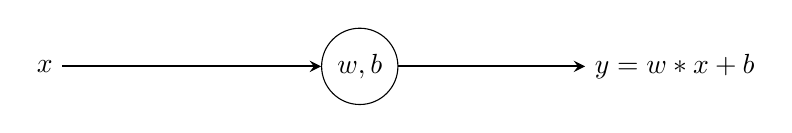
\begin{tikzpicture}

\node (x) at (-4,0) {$ x $};
\node (neuron) [draw,circle] at (0,0) {$ w,b $};
\node (y) at (4,0) {$ y = w*x + b $};
\draw [arrow] (x) -- (neuron);
\draw [arrow] (neuron) -- (y);
\end{tikzpicture}
\end{center}
\begin{block}{}
Where $ w $ is called the weight and $ b $ the bias. The idea is that we have an input $ x $ and an output $ y $, we want to find the linear relation between $ x $ and $ y $ so eventually find the correct $ w $ and $ b $.
\end{block}
\end{frame}

\begin{frame}
\frametitle{Neural Networks - Artificial Neurons}
\begin{block}{How to do this ?}
Using neural network's concepts called forward and backward propagation, in the forward propagation phase we calculate the output $ y^{\prime} = w*x ++ b $, backward propagation consists on calculating the loss between the real target $ y $ and the predicted target $ y^{\prime} $ and adjust the weight $ w $ and bias$ b $ and get closer to the correct values.
\end{block}
\begin{block}{How to adjust $ w $ and $ b $ ?}
The goal is to minimize the loss as between $ y^{\prime} $ and $ y $ as much as possible. Each time we calculate the loss we adjust the weight and bias using a specific optimizer, lets talk about one of these optimizers called Gradient Descent :
\end{block}
\end{frame}

\begin{frame}

\frametitle{Neural Networks - Gradient Descent Optimizer}
Consider the loss $ L(y,y^{\prime}) = L(w,b) $. So we adjust the weight and bias in this manner :\\
\begin{center}
$ w = w - \alpha*\dfrac{\partial L(w,b)}{\partial w} $ \hspace{1cm} and \hspace{1cm} $ b = b - \alpha*\dfrac{\partial L(w,b)}{\partial b} $
\end{center}
Where $ \alpha $ is what we call the learning rate which is a hyper parameter.
\begin{block}{Steps for adjustment of $ w $ and $ b $ using Gradient Descent}
\begin{itemize}
\item Step 1 : Randomly initialize $ w $ and $ b $
\item Step 2 : Calculate $ y^{\prime} = w*x + b $
\item Step 3 : Calculate the loss $ L(y,y^{\prime}) $
\item Step 4 : Adjust $ w $ and $ b $ as explained above
\item Step 5 : Repeat step 2 $ e $ times, where $ e $ is called the number of epochs
\end{itemize}
\end{block}

\end{frame}

\begin{frame}
\frametitle{Neural Networks - Gradient Descent}

\begin{example}
Linear regression, simplest regression problem, consider having 2 variables : input $ x = 1 $ and output $ y = 2 $ and we want to find the linear relation between them. We will consider a network having only one neuron with weight $ w $ and bias $ b $ with initial values equal to 0 for both with a learning rate $ \alpha = 1 $ and we will use as a loss function :\\
\begin{center}
$ L(y,y^{\prime}) = |y^{\prime} - y| $\\
\end{center}
At epoch 1 :
\begin{center}
$ y^{\prime} = w*x + b = 0*1 + 0 = 0 $ \hspace{5mm} so \hspace{5mm} $ y^{\prime} - y = 0 - 2 = -2 $ \hspace{5mm} which is negative\\
So \hspace{5mm} $ L(y,y^{\prime}) = L(w,b) = y - y^{\prime} = y - w*x - b $ \hspace{5mm} to get :
\end{center}

\end{example}

\end{frame}

\begin{frame}
\frametitle{Neural Networks - Gradient Descent}
\begin{example}
\begin{center}
$ \dfrac{\partial L(w,b)}{\partial w} = -x = -1 $ \hspace{5mm} and \hspace{5mm} $ \dfrac{\partial L(w,b)}{\partial b} = -1 $
\end{center}
\begin{center}
So lets adjust $ w $ and $ b $ :\\
$ w = w - \alpha*\dfrac{\partial L(w,b)}{\partial w} = 0 - 1*(-1) = 1 $ \hspace{5mm} and \hspace{5mm} $ b = b - \alpha*\dfrac{\partial L(w,b)}{\partial b} = 0 - 1*(-1) = 1 $\\
Epoch 1 is done.
\end{center}
\end{example}
\end{frame}

\begin{frame}
\frametitle{Neural Networks - Gradient Descent}
\begin{example}
At epoch 2 :
\begin{center}
$ y^{\prime} = w*x + b = 1*1 + 1 = 1 + 1 = 2 $ \hspace{5mm} and \hspace{5mm} $ y = 2 $\\
So \hspace{5mm} $ L(w,b) = L(y,y^{\prime}) = |y^{\prime} - y| = |2 - 2| = 0 $\\
And with a loss being equal to zero, out work here is done and the correct values are $ w = 1 $ and $ b = 1 $ so we get the linear relation between input and output : $ y = w*x + b = x + 1 $
\end{center}
\end{example}
\end{frame}

\begin{frame}
\frametitle{Neural Networks - Gradient Descent}
Now what would happen if we have a vector of input values and a vector of output values instead but still only one neuron?\\
In this case we will have to define a new hyper parameter called batch size. To understand the idea behind the batch size lets consider this example :

\begin{example}
Lets consider an input vector $ x $ of $ n $ values and an output vector $ y $  with a batch size $ = 3 $. the network will forward propagate each 3 values in the input vector and calculate the predicted output of each of them $ y^{\prime} $ then calculate the 3 losses for each of them and find there mean
\begin{center} 
$ loss = \dfrac{1}{3}\sum_{i=1}^{i=3}L_i(y,y^{\prime}) $
\end{center}
and adjust $ w $ and $ b $ using $ loss $, this process is called Stochastic Gradient Descent(SGD).
\end{example}
\end{frame}

\begin{frame}
\frametitle{Neural Networks - Gradient Descent}
\begin{block}{More complex}
Now if each value of the input vector is a vector it self of m values (input is a $ n*m $ matrix) but still one neuron, here $ w $ would be a vector of length $ m $ and $ b $ would still be one number.Lets consider $ m = 4 $ and that we are forward propagating the row $ i $ of the input matrix :\\
\end{block}
\end{frame}

\begin{frame}
\frametitle{Neural Networks - Gradient Descent}
\begin{center}
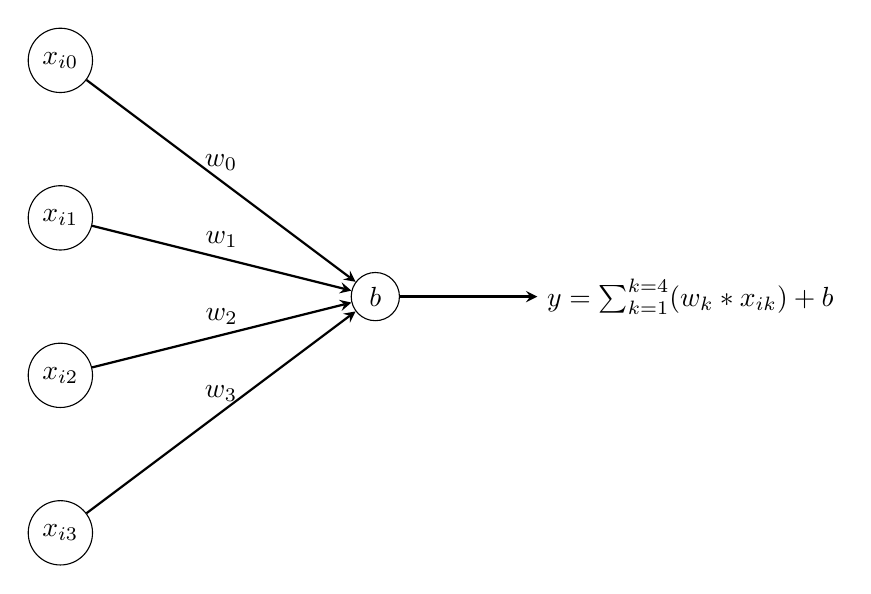
\begin{tikzpicture}

\node (x0) [draw,circle] at (-4,6) {$ x_{i0} $};
\node (x1) [draw,circle] at (-4,4) {$ x_{i1} $};
\node (x2) [draw,circle] at (-4,2) {$ x_{i2} $};
\node (x3) [draw,circle] at (-4,0) {$ x_{i3} $};
\node (neuron) [draw,circle] at (0,3) {$ b $};
\draw [arrow] (x0) -- node[anchor=south] {$ w_0 $} (neuron);
\draw [arrow] (x1) -- node[anchor=south] {$ w_1 $} (neuron);
\draw [arrow] (x2) -- node[anchor=south] {$ w_2 $} (neuron);
\draw [arrow] (x3) -- node[anchor=south] {$ w_3 $} (neuron);
\node (y) at (4,3) {$ y = \sum_{k=1}^{k=4}(w_k*x_{ik}) + b $};
\draw [arrow] (neuron) -- (y);

\end{tikzpicture}
\end{center}
\end{frame}

\begin{frame}
\frametitle{Neural Networks - Gradient Descent}
\begin{block}{In a more general way}
consider having an input matrix $ X $ of $ n $ instances with each instance being a vector of $ m $ values (matrix $ X $ size $ n*m $), and $ u $ neurons in one layer, the output of that layer would be a vector of length $ u $, $ w $ would be a matrix of size $ (m*u) $ and $ b $ a vector of $ u $ values. To calculate the output vector of this layer :\\
\begin{center}
$ \vec{y^{\prime}} = w^{T}*\vec{x} + \vec{b} $
\end{center}
\end{block}
\end{frame}

\begin{frame}
\frametitle{Neural Networks - Activation Functions}
\begin{block}{Non-linearity}
If a linear relationship does not exist between our input and output, we should introduce to our network some non-linearity using an activation function $ f $ , the output of our neuron would be just $ f( $output explained before adding the activation function$ ) $. Some of the famous activation functions used are:\\
\begin{itemize}
\item Relu : $ f(x) = max(0,x) $
\item Hyperbolic tangent : $ f(x) = \tanh(x) = \dfrac{2}{1 + e^{-2x}} - 1 $
\item Sigmoid : $ f(x) = \dfrac{1}{1 + e^{-x}} $
\item Softmax
\end{itemize}
\end{block}
\end{frame}

\begin{frame}
\frametitle{Neural Networks - Activation Functions}
\begin{columns}
\column{0.33\textwidth}
\centering
\begin{figure}
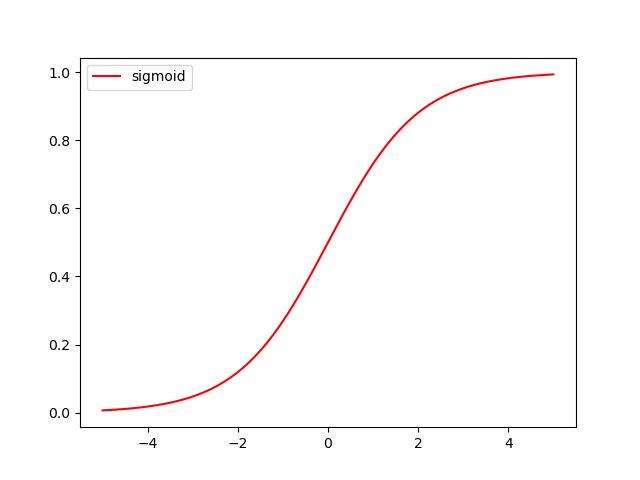
\includegraphics[scale=0.2]{sigmoid.png}
\caption{ - (a) Sigmoid}
\end{figure}
\column{0.33\textwidth}
\centering
\begin{figure}
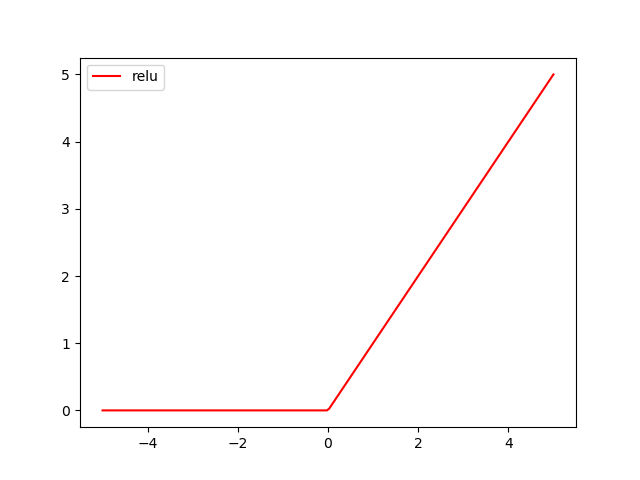
\includegraphics[scale=0.2]{relu.png}
\caption{ - (b) Relu}
\end{figure}
\column{0.34\textwidth}
\centering
\begin{figure}
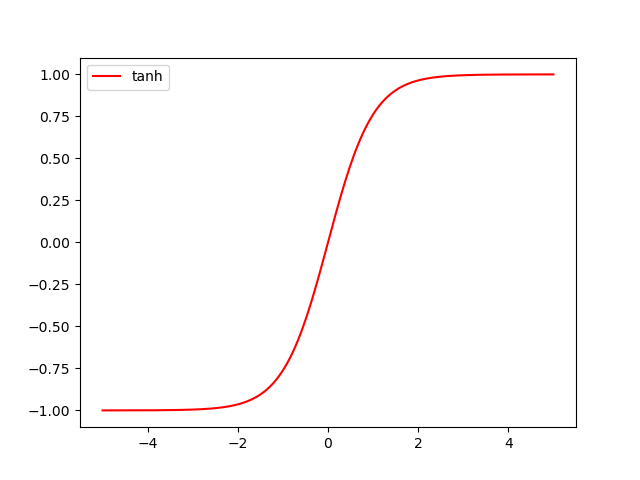
\includegraphics[scale=0.2]{tanh.png}
\caption{ - (c) Tanh}
\end{figure}
\end{columns}
\end{frame}

\begin{frame}
\frametitle{Neural Networks - Activation Functions - Softmax}
\begin{block}{Softmax activation function}
It is the most important key in solving a classification problem and its always used as an activation function for the last layer of the network. Softmax outputs a vector of probabilities :\\
Lets consider an ANN with $ n $ layers, where the $ n^{th} $ layer applies the softmax function, if $ x $ is the input of the last layer of length $ m $ and $ y $ its output of length $ k $ then :\\
Before applying softmax lets calculate the output $ \vec{u} = w^{T}*\vec{x} + \vec{b} $\\
\begin{center}
So : $ y_i = \dfrac{e^{u_i}}{\sum_{j=0}^{j=k}e^{u_j}} $
\end{center}
\end{block}

\end{frame}

\begin{frame}
\frametitle{Neural Networks - Activation Functions - Softmax}
Question : The predicted values for each instance is now a probability vector but our real value is only one number so how to calculate the loss between them ?\\
\begin{block}{Solution}
Transform all of our data set's real values vector into a binary matrix, for example if we had a vector of real targets $ [0,1,2,2] $ that means we only have three classes here 0, 1 and 2 then we would transform it to :
\begin{center}
$\begin{pmatrix}
1 & 0 & 0\\
0 & 1 & 0\\
0 & 0 & 1\\
0 & 0 & 1
\end{pmatrix}$
\end{center}
\end{block}
\end{frame}

\begin{frame}
\frametitle{Neural Networks - Activation Functions - Softmax}
Another question : What loss function should we use ?\\
\begin{block}{Solution}
The Categorical Cross-Entropy (CCE) loss :
\begin{center}
$ CCE = -\sum_{i=1}^{i=C}y_i*\log(y^{\prime}_i) $
\end{center}
$ C $ being the number of classes, $ y $ the target vector (a row from the matrix shown above) and $ y^{\prime} $ the output of the softmax layer.
\end{block}
\end{frame}

\begin{frame}
\frametitle{Neural Networks - Layers}
We have two categories of layers : hidden and non hidden layers.
\begin{block}{Non hidden layers :}
Only two exists :
\begin{itemize}
\item Input Layer : It is a must (no parameters involved)
\item Output Layer : It is a must (Usually with a softmax activation function with a number of units equal to the number of classes in our data set)
\end{itemize}
\end{block}
\begin{block}{Hidden layers :}
A lot of types exists but we will talk about the ones we used in our project
\begin{itemize}
\item \small Dense Layer
\item \small Max Pooling 2D Layer
\item \small 2D Convolution Layer (Conv2D)
\item \small Dropout Layer
\item \small Flatten Layer
\end{itemize}
\end{block}

\end{frame}

\begin{frame}
\frametitle{Neural Networks - Layers - Dense Layer}
The dense layer was explained before, it consists of having $ u $ neurons and one activation function $ f $ and its output (lets call it $ y $) is calculated in the following way :\\
\begin{center}
$ \vec{y} = f(w^{T}*\vec{x} + \vec{b}) $
\end{center}
$ w $ is a $ (n*u) $ matrix where $ n $ is the length of the input vector and $\vec{b} $ is a vector of length $ u $.
\end{frame}

\begin{frame}
\frametitle{Neural Networks - Layers - Max Pooling 2D Layer}
Its goal is just to reduce the size of its input.\\
\begin{example}
lets say you have a $ 4x4 $ matrix :\\
$D = 
\begin{pmatrix}
1 & 3 & 2 & 1\\
2 & 9 & 1 & 1\\
1 & 3 & 2 & 3\\
5 & 6 & 1 & 2
\end{pmatrix}
$
Then applying a $ (2,2) $ max pooling on it would produce :
$D^{\prime} = 
\begin{pmatrix}
9 & 2\\
6 & 3
\end{pmatrix}
$  Filter jumping 2 steps vertically and horizontally.
\end{example}
\end{frame}

\begin{frame}
\frametitle{Neural Networks - Layers - 2D Convolution Layer}
Here the filter jumps 1 step at the time regardless of the its size.\\
\begin{example}
Lets consider having the same matrix we used in the previous section about max pooling layer, using this matrix as a $ (2,2) $ filter :\\
$F = 
\begin{pmatrix}
1 & -1\\
-1 & 1
\end{pmatrix}
$
The first sub matrix the filter sees is : 
$A = 
\begin{pmatrix}
1 & 3\\
2 & 9
\end{pmatrix}
$\\
So to calculate the after filtering results we compute this :\\
\begin{center}
$ B = \sum_{i=1}^{i=2}F_i*A_i $
\end{center}
And we keep moving the filter around till we get a new matrix, for the above example the after filtering results would be :\\
$D^{\prime} = 
\begin{pmatrix}
5 & -7 & -1\\
-5 & -9 & 1\\
-1 & -4 & 0
\end{pmatrix}
$
\end{example}
\end{frame}

\begin{frame}
\frametitle{Neural Networks - Layers - Dropout Layer}
\begin{figure}
\centering
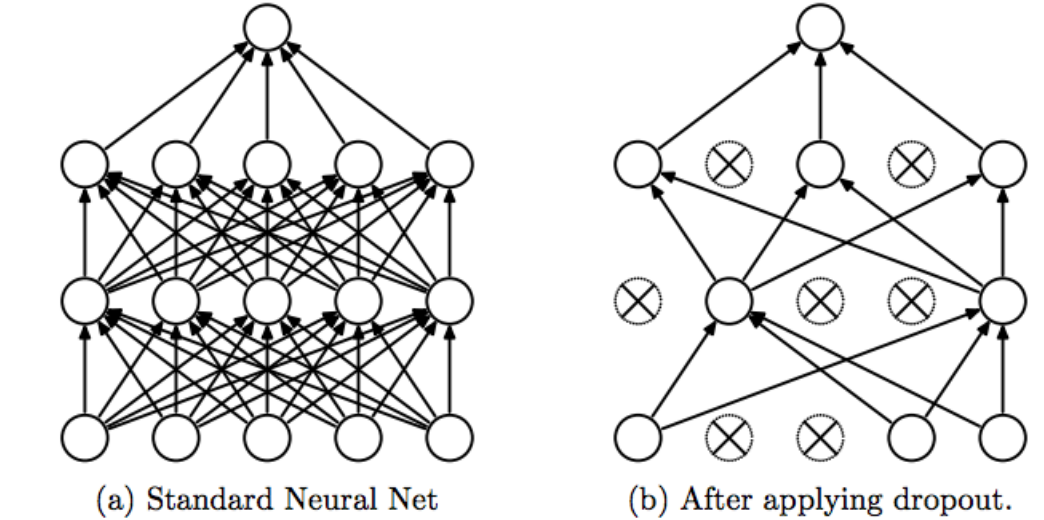
\includegraphics[scale=0.3]{dropout.png}
\caption{rivastava, Nitish, et al. ”Dropout: a simple way to prevent neural networks from
overfitting”, JMLR 2014}
\end{figure}
\end{frame}

\begin{frame}
\frametitle{Neural Networks - Layers - Flatten Layer}
\begin{block}{}
This layer does not have any parameters and it just takes the output of a hidden layer or input layer and transforms its data to a 1 dimensional vector .
\end{block}
\end{frame}

\section{Putting It All Together}

\begin{frame}
\frametitle{Putting It All Together}
\begin{block}{Implementation}
For the project we used :
\begin{itemize}
\item Python programming language using Visual Studio Code Text Editor
\item Tkinter Python module to implement the Graphical User Interface (GUI)
\item Sklearn Python module to get the Euclidean Distances and calculate the score of our evaluations
\item Tslearn Python module to get the Dynamic Time Warping Distances
\item Keras Python Module to implement our neural network
\item Matplotlib Python Module to plot the loss, accuracy and draw all the plots used in this presentation.
\item Texmaker software to write the presentation and report using Latex language
\end{itemize}

\end{block}
\end{frame}

\begin{frame}
\frametitle{Putting It All Together}
\begin{figure}
\centering
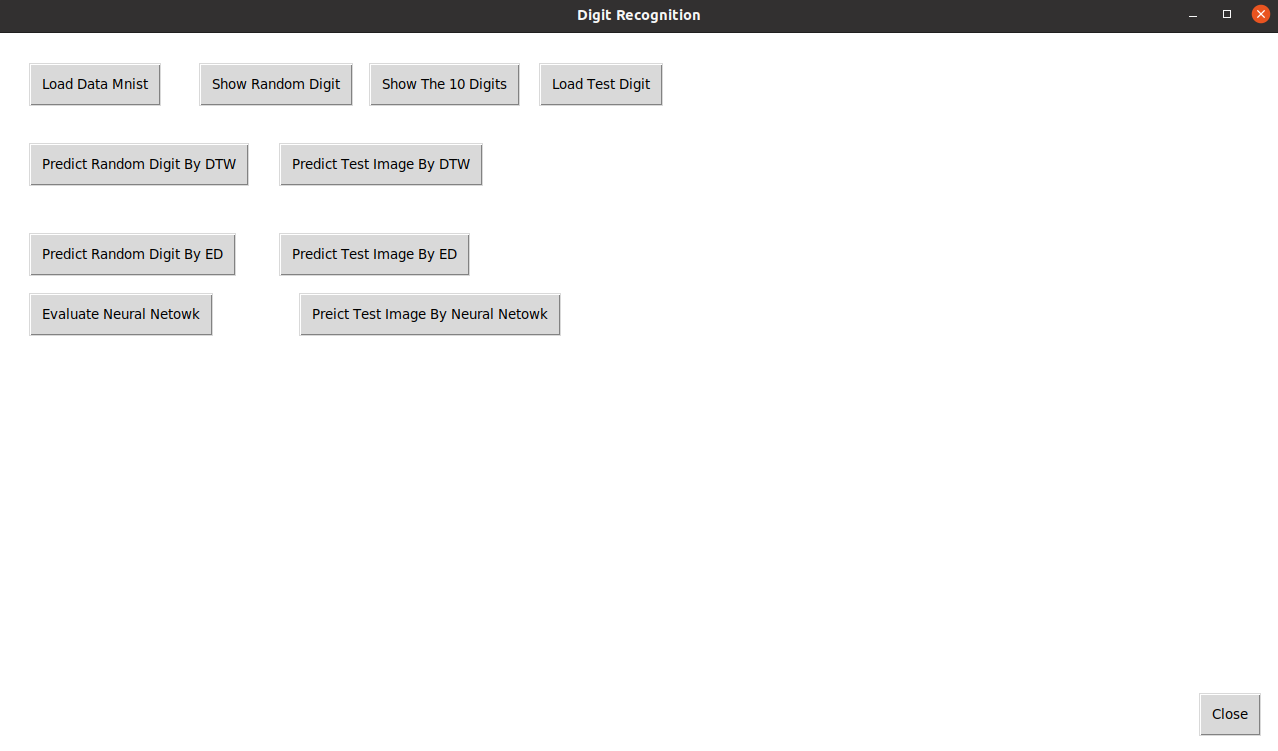
\includegraphics[scale=0.25]{MY_GUI.png}
\end{figure}
\end{frame}

\begin{frame}
\frametitle{Putting It All Together}
\begin{block}{Our Neural Network has the following architecture :}
\begin{itemize}
\item Layer 1 : Input layer
\item Layer 2 : Conv2D layer, number of filters is 32 and kernel size is (3,3), relu activation function
\item Layer 3 : Conv2D layer, number of filters is 64 and kernel size is (3,3), relu activation function
\item Layer 4 : MaxPool2D layer, pool size is (2,2)
\item Layer 5 : Dropout layer, with a keep probability of 25\%
\item Layer 6 : Flatten layer
\item Layer 7 : Dense layer, 128 units with a relu activation function
\item Layer 8 : Dropout layer, with a keep probability of 50\%
\item Layer 9 : Output Dense layer, 10 units with a softmax activation function
\end{itemize}
\end{block}
\end{frame}

\section{Results}

\begin{frame}
\frametitle{Results}
\begin{center}
\begin{tabular}{|p{2cm}||p{2cm}|p{2cm}|p{2cm}|p{2cm}|}
\hline
\multicolumn{5}{|c|}{Neural Network Results} \\
\hline
Optimizer & Batch Size & Learning Rate & Number of Epochs & Test Accuracy\\
\hline
SGD & 128 & 0.01 & 10 & 96.42\%\\
\hline
SGD & 128 & 0.001 & 10 & 91.92\%\\
\hline
SGD & 512 & 0.01 & 10 & 94.21\%\\
\hline
Adam & 128 & 0.01 & 10 & 98.72\%\\
\hline
Adam & 128 & 0.001 & 10 & 99.02\%\\
\hline
Adam & 512 & 0.01 & 10 & 98.81\%\\
\hline
Adadelta & 128 & 0.01 &10 & 93.63\%\\
\hline
Adadelta & 128 & 0.001 &10 & 81.55\%\\
\hline
Adadelta & 512 & 0.01 &10 & 91.15\%\\
\hline
\end{tabular}
\end{center}
\end{frame}

\begin{frame}
\frametitle{Results}
\begin{center}
\begin{tabular}{|p{4.3cm}||p{2cm}|p{2cm}|p{2cm}|}
\hline
\multicolumn{4}{|c|}{Nearest Neighbor Results}\\
\hline
Distance & Train set size & Test set size & Test accuracy\\
\hline
Euclidean & 200 & 100 & 75\%\\
\hline
Dynamic Time Warping & 200 & 100 & 83\%\\
\hline
\end{tabular}
\end{center}
\end{frame}

\section{Discussion}

\begin{frame}
\frametitle{Discussion}
\begin{block}{Observations}
\begin{itemize}
\item DTW is better than ED but slower
\item There isn't one best way using the neural network method
\item The best optimizer for our data and network architecture is Adam with a learning rate of 0.001, batch size of 128 and number of epochs of 10
\end{itemize}
\end{block}
\begin{alertblock}{Note}
Of course there can be better ways for this architecture and data set.
\end{alertblock}
\end{frame}

\section{Conclusion}
\begin{frame}
\frametitle{Conclusion}
\begin{itemize}
\item Neural networks are the best way to build AI machines (for now)
\item Big number of hyper parameters so it takes time to find the best way
\item The hardware is very important for the time of training
\item Neural networks can learn just like humans do
\item Always find different results and compare 
\item Can we trust AI ?
\end{itemize}
\end{frame}

\section{References}

\begin{frame}
\frametitle{References}
\begin{itemize}

\item \textcolor{blue}{\url{https://becominghuman.ai/introduction-to-artificial-intelligence-5fba0148ec99}}
\item \textcolor{blue}{\url{https://www.overleaf.com/learn/latex}}
\item \textcolor{blue}{\url{https://medium.com/@urvashilluniya/why-data-normalization-is-necessary-for-machine-learning-models-681b65a05029}}
\item \textcolor{blue}{\url{https://towardsdatascience.com/understand-data-normalization-in-machine-learning-8ff3062101f0}}
\item \textcolor{blue}{\url{https://medium.com/datadriveninvestor/k-nearest-neighbors-knn-7b4bd0128da7}}
\item \textcolor{blue}{\url{https://medium.com/@srishtisawla/k-nearest-neighbors-f77f6ee6b7f5}}

\end{itemize}
\end{frame}

\begin{frame}
\frametitle{References}
\begin{itemize}
\item \textcolor{blue}{\url{https://medium.com/datadriveninvestor/dynamic-time-warping-dtw-d51d1a1e4afc}}
\item \textcolor{blue}{\url{https://towardsdatascience.com/dynamic-time-warping-3933f25fcdd}}
\item \textcolor{blue}{\url{https://medium.com/@purnasaigudikandula/a-beginner-intro-to-neural-networks-543267bda3c8}}
\item \textcolor{blue}{\url{https://mathanrajsharma.medium.com/softmax-activation-function-e582ea53ada7}}
\item \textcolor{blue}{\url{https://medium.com/fintechexplained/neural-network-layers-75e48d71f392}}
\item \textcolor{blue}{\url{https://gombru.github.io/2018/05/23/cross_entropy_loss/}}
\end{itemize}
\end{frame}

\begin{frame}
\frametitle{References}
\begin{itemize}
\item \textcolor{blue}{\url{https://medium.com/datathings/dense-layers-explained-in-a-simple-way-62fe1db0ed75}}
\item \textcolor{blue}{\url{https://medium.com/@brightonnkomo/convolutional-neural-networks-part-4-the-pooling-and-fully-connected-layer-394ec01fb00d}}
\item \textcolor{blue}{\url{https://xzz201920.medium.com/conv1d-conv2d-and-conv3d-8a59182c4d6}}
\item \textcolor{blue}{\url{https://medium.com/@amarbudhiraja/https-medium-com-amarbudhiraja-learning-less-to-learn-better-dropout-in-deep-machine-learning-74334da4bfc5}}
\item \textcolor{blue}{\url{https://towardsdatascience.com/the-most-intuitive-and-easiest-guide-for-convolutional-neural-network-3607be47480}}
\end{itemize}
\end{frame}

\begin{frame}
\frametitle{References}
\begin{itemize}
\item \textcolor{blue}{\url{https://keras.io/}}
\item \textcolor{blue}{\url{https://scikit-learn.org/stable/}}
\item \textcolor{blue}{\url{https://tslearn.readthedocs.io/en/stable/}}
\item \textcolor{blue}{\url{https://numpy.org/}}
\item \textcolor{blue}{\url{https://matplotlib.org/}}
\item \textcolor{blue}{\url{https://docs.python.org/3/library/tkinter.html}}
\item \textcolor{blue}{\url{https://docs.python.org/3/}}

\end{itemize}
\end{frame}

\begin{frame}{END}
\begin{center}
\Huge THANK YOU FOR YOUR TIME
\end{center}
\end{frame}

\end{document}